% !TeX spellcheck = cs_CZ
%{\tikzset{external/prefix={tikz/FYZI/}}
% \tikzset{external/figure name/.add={ch20_}{}}
%---------------------------------------------------------------------------------------------------
% file fey1ch20.tex
%---------------------------------------------------------------------------------------------------
%=========================== Kapitola: Rotace v prostoru ===========================================
\chapter{Rotace v prostoru}\label{fyz:IchapXX}
\minitoc
  \section{Momenty sil v prostoru}\label{fyz:IchapXXsecI}
  \section{Rovnice rotace a vektorový součin}\label{fyz:IchapXXsecII}
  \section{Setrvačník}\label{fyz:IchapXXsecIII}
  \section{Moment hybnosti tuhého tělesa}\label{fyz:IchapXXsecIV}
  \section{Příklady a cvičení}\label{fyz:IchapXXsecV}  

  \begin{figure}[ht!] %\ref{fyz:fig406}
    \centering
    \begin{tabular}{cc}
     \subfloat[ ]{\label{fyz:fig406a}
       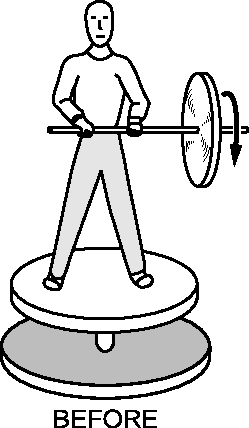
\includegraphics[width=0.45\linewidth]{fyz_fig406a.pdf}} 
     \subfloat[ ]{\label{fyz:fig406b}
       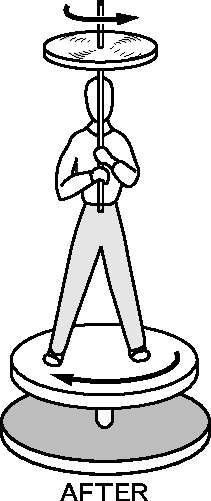
\includegraphics[width=0.45\linewidth]{fyz_fig406b.pdf}}
    \end{tabular}
    \caption{a) osa má horizontální směr; moment hybnosti vzhledem k vertikální ose je roven nule 
             b) osa má vertikální směr; moment hybnosti vzhledem k vertikální ose je stále roven 
             nule; člověk a žídle se otáčejí v opačném směru než kolo
             (\cite[s.~278]{Feynman01}).}
    \label{fyz:fig406}
  \end{figure}

  \begin{figure}[ht!] %\ref{fyz_fig407}
    \centering
    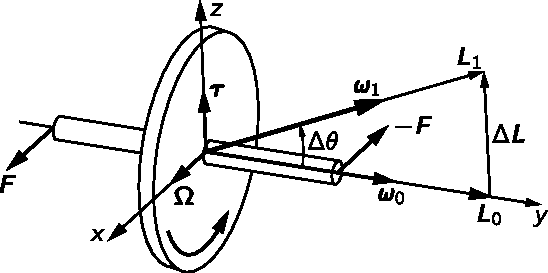
\includegraphics[width=0.3\linewidth]{fyz_fig407.pdf}
    \caption{Setrvačník
             (\cite[s.~279]{Feynman01})}
    \label{fyz_fig407}
  \end{figure}

  \begin{figure}[ht!] %\ref{fyz_fig408}
    \centering
    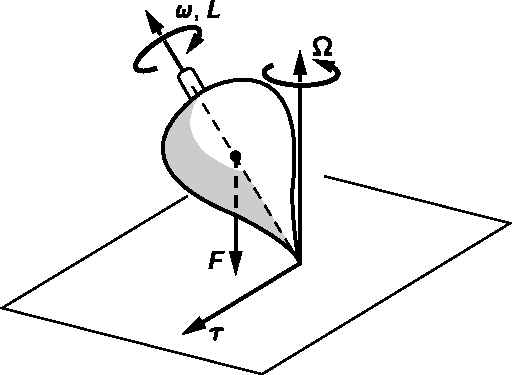
\includegraphics[width=0.3\linewidth]{fyz_fig408.pdf}
    \caption{Rychle se otáčející káča. Směr vektoru momentu síly je směrem precese 
             (\cite[s.~280]{Feynman01})}
    \label{fyz_fig408}
  \end{figure}

  \begin{figure}[ht!] %\ref{fyz_fig409}
    \centering
    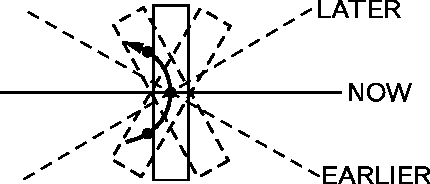
\includegraphics[width=0.3\linewidth]{fyz_fig409.pdf}
    \caption{Při otáčení osy vykonávají částice rotujícího kola (obr. \ref{fyz_fig407}) pohyb, 
             který se děje po zakřivených trajektoriích 
             (\cite[s.~280]{Feynman01})}
    \label{fyz_fig409}
  \end{figure}

  \begin{figure}[ht!] %\ref{fyz_fig410}
    \centering
    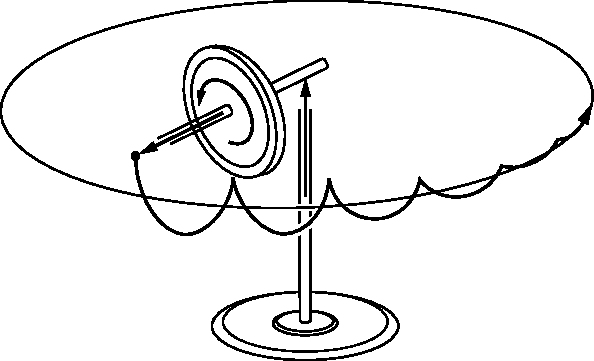
\includegraphics[width=0.3\linewidth]{fyz_fig410.pdf}
    \caption{Skutečný pohyb konce setrvačníku pod vlivem tíhy ihned po uvolnění předtím uchycené osy
             (\cite[s.~281]{Feynman01})}
    \label{fyz_fig410}
  \end{figure}

  \begin{figure}[ht!] %\ref{fyz_fig411}
    \centering
    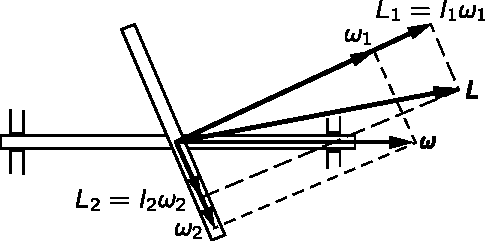
\includegraphics[width=0.3\linewidth]{fyz_fig411.pdf}
    \caption{Moment hybnosti rotujícího tělesa není nutně rovnoběný s úhlovou rychlostí
             (\cite[s.~282]{Feynman01})}
    \label{fyz_fig411}
  \end{figure}

  \begin{figure}[ht!] %\ref{fyz_fig412}
    \centering
    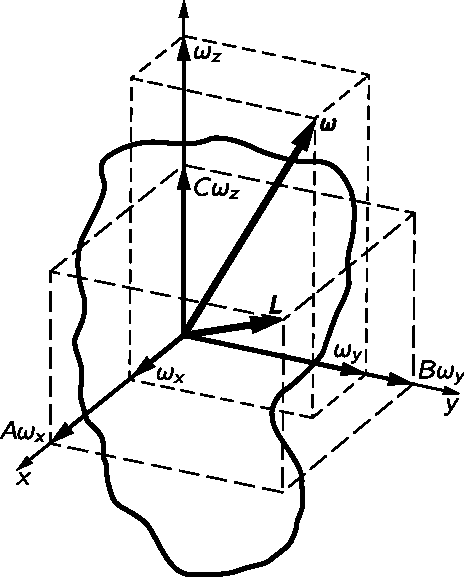
\includegraphics[width=0.3\linewidth]{fyz_fig412.pdf}
    \caption{Úhlová rychlost a moment hybnosti tuhého tělesa (\(A>B>C\))
             (\cite[s.~283]{Feynman01})}
    \label{fyz_fig412}
  \end{figure}
  
%} %tikzset
%---------------------------------------------------------------------------------------------------
\printbibliography[title={Seznam literatury}, heading=subbibliography]
\addcontentsline{toc}{section}{Seznam literatury}